\par \indent Diagnosis identifies outliers in the time course according to
three measures: volume standard deviation values, RMS difference values, and
extended difference values. The script returns plots for the volume standard
deviation values [Figure \ref{fig:vol_std}], the RMS vector [Figure \ref{fig:rms}], and the extended RMS vector [Figure \ref{fig:erms}]. Outliers are labeled as red dots in the figures.

\begin{figure}[h!]
\centering
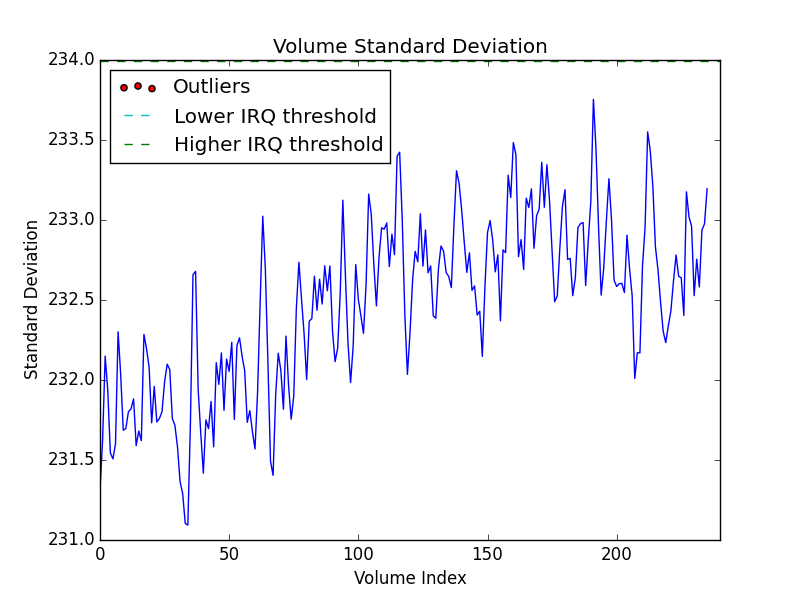
\includegraphics[width=120mm]{images/vol_std.png}
\caption{volume standard deviation for Subject 1 in Run 1}
\label{fig:vol_std}
\end{figure}

\begin{figure}[h!]
\centering
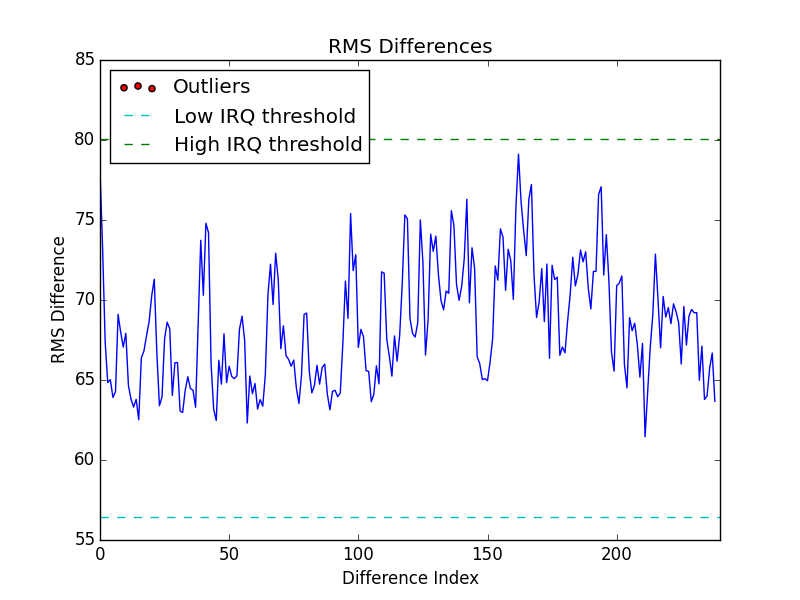
\includegraphics[width=120mm]{images/vol_rms_outliers.png}
\caption{RMS difference values for Subject 1 in Run 1}
\label{fig:rms}
\end{figure}

\begin{figure}[h!]
\centering
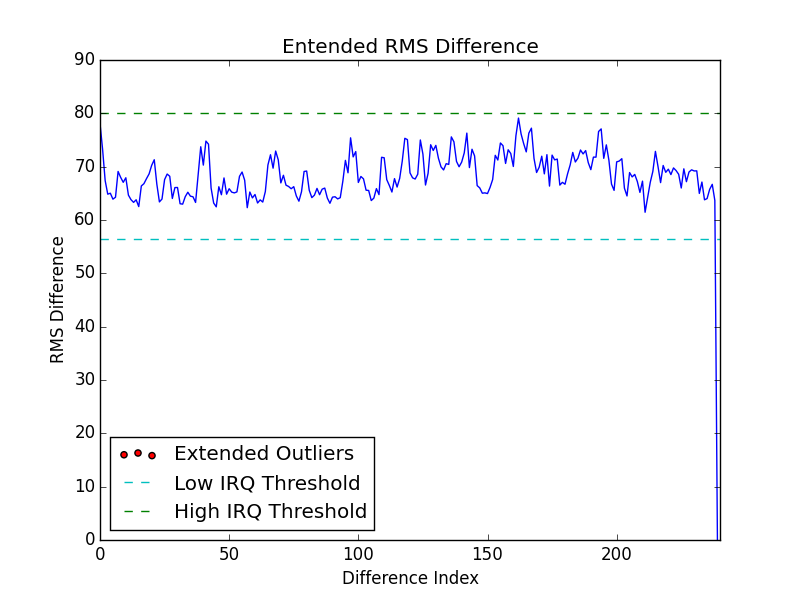
\includegraphics[width=120mm]{images/extended_vol_rms_outliers.png}
\caption{Extended RMS difference values for Subject 1 in Run 1}
\label{fig:erms}
\end{figure}
